% !TeX TS-program = lualatex
\documentclass[aspectratio=169]{beamer}

% Use a clean default theme to match the uploaded document
\usetheme{default}
\usecolortheme{default}

\usepackage{graphicx}
\usepackage{amsmath}
\usepackage{amssymb} % For checkmarks
\usepackage{caption}

\usefonttheme{professionalfonts} % using non standard fonts for beamer
\usefonttheme{serif} % default family is serif
\usepackage{fontspec}
\setmainfont{Ubuntu}

% ---------------------------------------------------------
% Customizing the Style to match the uploaded PDF
% ---------------------------------------------------------
\definecolor{mygrey}{RGB}{250, 248, 237}
% Change slide background color
\setbeamercolor{background canvas}{bg=mygrey}

% 1. Custom Footer for ALL pages
\setbeamertemplate{footline}{
    \leavevmode%
    \hbox{%
    \begin{beamercolorbox}[wd=\paperwidth,ht=3ex,dp=1.5ex,center]{footline}%
        \tiny Kibrom E. \hspace{12em} Mekelle University | School of Electrical \& Computer Engineering \hspace{12em} \insertframenumber
    \end{beamercolorbox}}%
    \vskip3pt%
}

% 2. Remove default navigation symbols at the bottom right
\setbeamertemplate{navigation symbols}{}

% 3. Clean Frame Titles with an underline
\setbeamertemplate{frametitle}{
    \vspace{0.4cm}
    {\Large \textbf{\insertframetitle}} \par
    \vspace{0.1cm}
    \hrule
}

% 4. Custom Title Page Layout (Centered, Logo on top)
\setbeamertemplate{title page}{
    \begin{center}
        \vspace{0.3cm}
        % Logo at the top
        
\includegraphics[height=3cm]{img/logo.jpg} \\ 
        \vspace{0.4cm}
        
        % Main Title
        {\Large \textbf{\inserttitle}} \\
        \vspace{0.4cm}
        
        % Subtitle
        {\textbf{Mekelle University\\
            Ethiopian Institute of Technology-Mekelle (EiT-M)\\
            School of Electrical and Computer Engineering\\
            Industrial Control Chair}} \\
        \vspace{0.3cm}
        
        % Author and Advisor
        {\normalsize \textbf{Author:} Kibrom Esayas \quad | \quad \textbf{Advisor:} Dr.-Ing. Gebremicheal Te-ame} \\
        \vspace{0.2cm}
        
    \end{center}
}

% Title Data
\title[MPC of Active VSR]{Model Predictive Control of Active VSR Output Voltage under Unbalanced Grid Conditions}

\begin{document}

% ---------------------------------------------------------
% 1. Title Slide
% ---------------------------------------------------------
\begin{frame}
    \titlepage
\end{frame}

% ---------------------------------------------------------
% 2. Outline Slide (using checkmarks as seen in your PDF)
% ---------------------------------------------------------
\begin{frame}{Presentation Outline}
    \begin{itemize}
        \item[\checkmark] Introduction
        \item[\checkmark] Literature Review 
        \item[\checkmark] Problem Statement \& Objectives
        \item[\checkmark] Scope of the Thesis 
        \item[\checkmark] System Modeling
        \item[\checkmark] Controller Design (PI \& MPC)
        \item[\checkmark] Simulation Results \& Discussion
        \item[\checkmark] Conclusion \& Future Work
        \item[\checkmark] Q\&A Session
    \end{itemize}
\end{frame}

% ---------------------------------------------------------
\section{Introduction}
% ---------------------------------------------------------

% 3. Background
\begin{frame}{Background: Power Converters}
    Power electronic converters are essential for modern energy transformation, processing voltage/current to meet load requirements. Three-phase Active VSRs are specifically critical for:
    \vspace{0.3cm}
    \begin{itemize}
        \item \textbf{EV Charging:} High-power fast charging stations require stable DC output.
        \item \textbf{Renewable Energy:} Interfacing wind/solar systems with the conventional AC grid.
        \item \textbf{Industrial Drives:} High-efficiency motor control and power supplies.
    \end{itemize}
\end{frame}

% 4. VSC Topology
\begin{frame}{Three-Phase Active VSR Topology}
    \begin{columns}
        \column{0.5\textwidth}
        The standard topology features:
        \begin{itemize}
            \item \textbf{AC Side:} Input inductors (L) for current filtering and voltage boost.
            \item \textbf{Switching Bridge:} Six active switches (IGBTs) for PWM control.
            \item \textbf{DC Side:} Link capacitor (C) for voltage stiffening and energy storage.
        \end{itemize}
        
        \column{0.5\textwidth}
        \begin{figure}
            \centering
            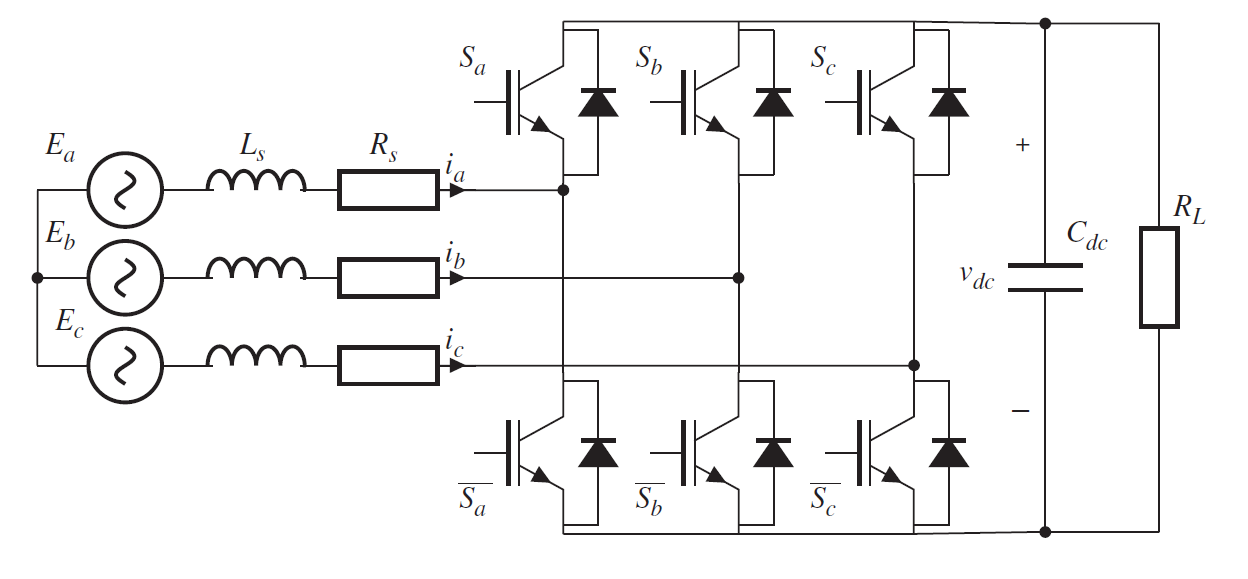
\includegraphics[width=\textwidth]{img/twolevelvsctopology.png}
            \caption{Three-Phase Active VSR Topology}
        \end{figure}
    \end{columns}
\end{frame}

% ---------------------------------------------------------
\section{Literature Review}
% ---------------------------------------------------------

% Literature Review Slide 1
\begin{frame}{Literature Review: Classical Control}
    Extensive research has been conducted on topologies and linear control schemes to manage unbalanced grid conditions:
    \vspace{0.3cm}
    \begin{itemize}
        \item \textbf{Dual Current Control:} H.-s. Song and K. Nam, addresses the issue where
            voltage unbalance causes 2$\omega$ ripples in the DC-link voltage and increases reactive power. They
            proposed a dual current control scheme using two synchronous reference frames (SRF): one
            rotating counter-clockwise for the positive sequence and one clockwise for the negative sequence.
            by filtering out the oscillating components in each frame, to achieve ripple-free DC voltage and unity power factor.
    \end{itemize}
\end{frame}

\begin{frame}{Literature Review: Classical Control \dots(Cont'd) }
    \vspace{0.3cm}
    \begin{itemize}
        \item \textbf{Sequence Extraction:} M. Mirhosseini discuss the stability restrictions
            of PI parameters when using Moving Average Filters (MAF) to extract sequence components.
            The delay introduced by filtering techniques slows down the dynamic response of the system,
            creating a tradeoff between stability regions and fast dynamic performance.
        \item \textbf{Voltage Support Optimization:} Camacho et al. explores strategies to maximize voltage
            support during grid faults. They developed optimal solutions to maximize positive sequence
            voltage or minimize negative sequence voltage while injecting maximum rated current. Their
            work highlights that optimal power reference generation depends heavily on the grid impedance
            (L/R ratio), which can vary widely in real-world conditions.
    \end{itemize}
\end{frame}

% Literature Review Slide 2
\begin{frame}{Literature Review: Limitations of Linear Controllers}
    Despite their simplicity, traditional Proportional-Integral (PI) controllers face significant
    challenges under asymmetrical fault conditions:
    \vspace{0.3cm}
    \begin{itemize}
        \item \textbf{Dynamic Stability:} PI controllers struggle to maintain stability margins when 
        exposed to rapid, dynamic fault transients.
        \item \textbf{Filtering Delays:} Accurately extracting sequence components requires extensive 
        filtering (e.g., Moving Average Filters or Notch Filters).
        \item \textbf{The Core Trade-off:} These filters inherently introduce severe time delays. 
        This creates an unavoidable trade-off between isolating the $2\omega$ oscillations and maintaining
        a fast dynamic response.
    \end{itemize}
\end{frame}

% Literature Review Slide 3
\begin{frame}{Literature Review: MPC }
    \begin{itemize}
        \item \textbf{Finite control set MPC:} Wang et al. explores an MPC strategy that directly
            controls the output voltage of a three-phase VSR under unbalanced conditions. Their approach
            involves predicting the future states of the system and optimizing the switching actions to
            minimize voltage deviations and harmonic distortion.\\
            \vspace{0.3cm}
            N. Jin, L. Guo proposed an MPC with direct power control scheme that incorporates a cost function designed to minimize
            both the output voltage error and the switching losses. Their results demonstrate that MPC
            can achieve superior voltage regulation and reduced harmonic content compared to classical PI
            controllers.
        \item \textbf{Previous MPC Limitations:} Existing MPC based control schemes often suffer from 
        variable switching frequencies which can lead to increased harmonic distortion and reduced system efficiency.
    \end{itemize}
\end{frame}  

% 4. Problem Statement
\begin{frame}{Statement of the Problem}
    Grid voltages are rarely ideal. Asymmetrical faults create significant performance issues for standard VSRs:
    \vspace{0.3cm}
    \begin{itemize}
        \item \textbf{The Core Issue:} Negative sequence voltage components create oscillating power terms at $2\omega$ (twice the fundamental frequency).
        \item \textbf{DC Link Ripple:} Continuous fluctuation at twice the grid frequency.
        \item \textbf{Harmonic Distortion:} Non-sinusoidal AC currents violating power quality standards.
        \item \textbf{Thermal Stress:} Excessive heating in semiconductor components due to current imbalance.
    \end{itemize}
\end{frame}

% 5. Objectives
\begin{frame}{Research Objectives}
    \textbf{General Objective:}\\
    Design a Model Predictive Control (MPC) strategy for a three-phase active VSR to achieve regulated output voltage and suppress ripples under unbalanced grid conditions.
    
    \vspace{0.5cm}
    \textbf{Specific Objectives:}
    \begin{itemize}
        \item \textbf{Modeling:} Adopt a symmetrical sequence mathematical model.
        \item \textbf{Prediction:} Develop a discretized prediction model for the energy state.
        \item \textbf{Suppression:} Design a cost function for active ripple cancellation.
    \end{itemize}
\end{frame}

% ---------------------------------------------------------
\section{System Model}
% ---------------------------------------------------------

% 6. VSC Topology
\begin{frame}{Three-Phase Active VSR Mathematical Model}
    The voltage equations for the 3-phase system are given by:
\begin{equation*}
    \begin{gathered}
        e_{a} = L \frac{di_a}{dt} + R i_a + \mathcal{V}_a\\
        e_{b} = L \frac{di_b}{dt} + R i_b + \mathcal{V}_b\\
        e_{c} = L \frac{di_c}{dt} + R i_c + \mathcal{V}_c
    \end{gathered}
\end{equation*}
where $e_{a,b,c}$ are the grid voltages, $i_{a,b,c}$ are the phase currents and 
\begin{equation*}
    \begin{gathered}
        \mathcal{V}_a = S_a V_{dc} + V_{cm}\\
        \mathcal{V}_b = S_b V_{dc} + V_{cm}\\
        \mathcal{V}_c = S_c V_{dc} + V_{cm}
    \end{gathered}
\end{equation*}
\end{frame}

% 7. Symmetrical Components
\begin{frame}{Symmetrical Sequence Decomposition}
    \begin{columns}
        \column{0.5\textwidth}
        For unbalanced analysis, components are decomposed into Positive (p), Negative (n) and Zero (0) sequence networks:
        \begin{equation*}
            X_{abc} = X_{abc}^{p} + X_{abc}^{n} + X_{abc}^{0}
        \end{equation*}
        This allows decoupling the control for balanced and unbalanced terms independently.
        
        \column{0.5\textwidth}
        \begin{figure}
            \centering
            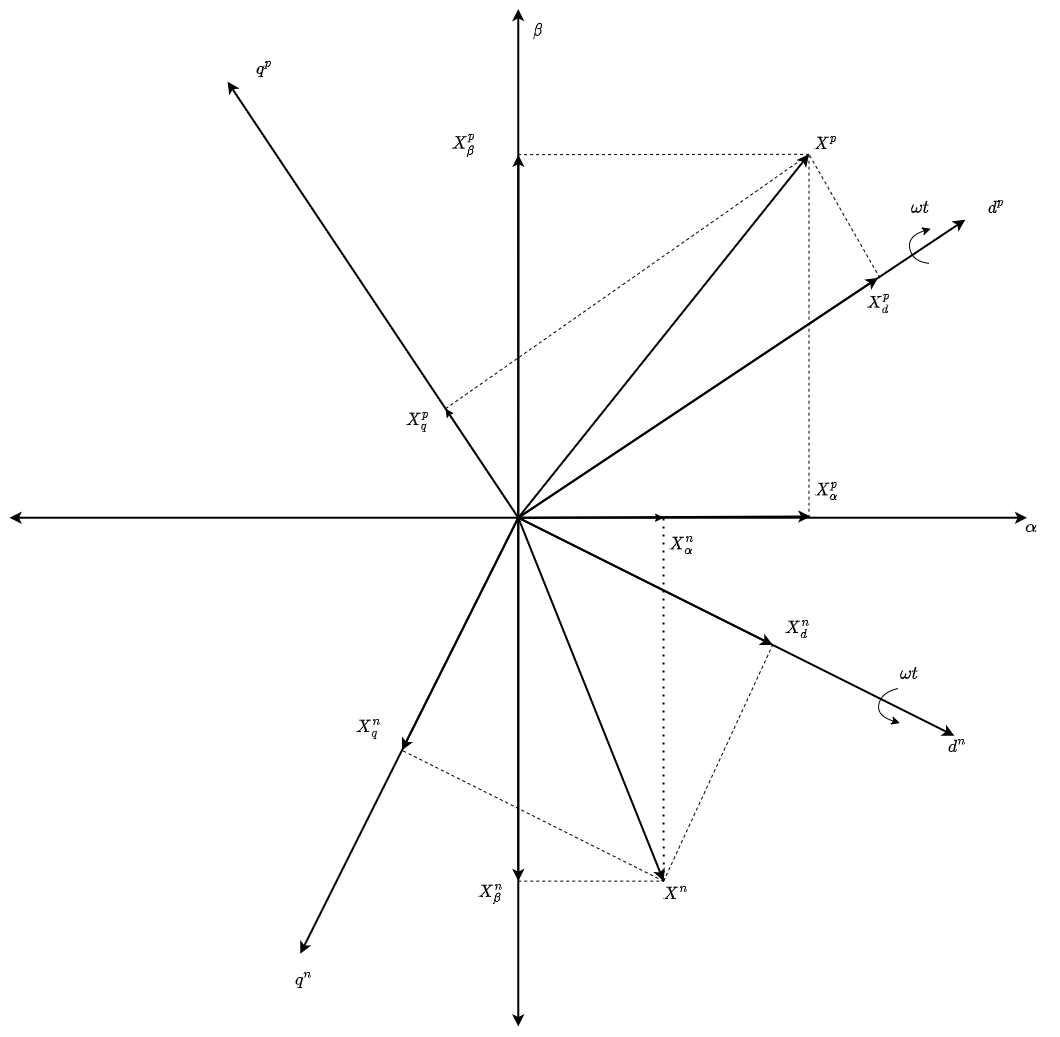
\includegraphics[width=0.9\textwidth]{img/symmetricalDecomposition.png}
        \end{figure}
    \end{columns}
\end{frame}

% 8. alpha-beta model
\begin{frame}{$\alpha$-$\beta$ and $d-q$ Mathematical Model}
    By applying the Clarke and Park transformations, the system can be represented in the $\alpha$-$\beta$
    stationary reference frame and the $d$-$q$ synchronous reference frame. The voltage equations are:
    \vspace{0.4cm}
    \begin{columns}
        \column{0.5\textwidth}
    \begin{equation*}
        \begin{gathered}
            e^{p}_{\alpha} =  L  \frac{d}{dt} i^{p}_{\alpha} + R i^{p}_{\alpha} + \mathcal{V}^{p}_{\alpha} \\
            e^{p}_{\beta} =  L  \frac{d}{dt} i^{p}_{\beta} + R i^{p}_{\beta} + \mathcal{V}^{p}_{\beta} \\
            e^{n}_{\alpha} =  L  \frac{d}{dt} i^{n}_{\alpha} + R i^{n}_{\alpha} + \mathcal{V}^{n}_{\alpha} \\
            e^{n}_{\beta} =  L  \frac{d}{dt} i^{n}_{\beta} + R i^{n}_{\beta} + \mathcal{V}^{n}_{\beta}
        \end{gathered}
    \end{equation*}

    \column{0.5\textwidth}
    \begin{equation*}
        \begin{gathered}
            e^{p}_{d} =  L  \frac{d}{dt} i^{p}_{d} + R i^{p}_{d} - \omega L i^{p}_{q} + \mathcal{V}^{p}_{d} \\
            e^{p}_{q} =  L  \frac{d}{dt} i^{p}_{q} + R i^{p}_{q} + \omega L i^{p}_{d} + \mathcal{V}^{p}_{q} \\
            e^{n}_{d} =  L  \frac{d}{dt} i^{n}_{d} + R i^{n}_{d} + \omega L i^{n}_{q} + \mathcal{V}^{n}_{d} \\
            e^{n}_{q} =  L  \frac{d}{dt} i^{n}_{q} + R i^{n}_{q} - \omega L i^{n}_{d} + \mathcal{V}^{n}_{q}
        \end{gathered}
    \end{equation*}
    \end{columns}
\end{frame}

% 9. Effect of unbalanced grid
\begin{frame}{Effect of Unbalanced Grid Voltages}
    Under unbalanced grid conditions the input apparent power of the system can be expressed as:
    \begin{equation*}
        \begin{split}
            S(t) &= \frac{3}{2}(e_{\alpha} + je_{\beta})(i_{\alpha} + ji_{\beta})^{*} \\
            S(t) &= \frac{3}{2}\Big[ \big(e_{d}^{p}\cos(\omega t) - e_{q}^{p}\sin(\omega t) + e_{d}^{n}\cos(\omega t) + e_{q}^{n}\sin(\omega t)\big) \\
            &\quad + j\big(e_{d}^{p}\sin(\omega t) + e_{q}^{p}\cos(\omega t) - e_{d}^{n}\sin(\omega t) + e_{q}^{n}\cos(\omega t)\big) \Big] \\
            &\quad \times \Big[ \big(i_{d}^{p}\cos(\omega t) - i_{q}^{p}\sin(\omega t) + i_{d}^{n}\cos(\omega t) + i_{q}^{n}\sin(\omega t)\big) \\
            &\quad - j\big(i_{d}^{p}\sin(\omega t) + i_{q}^{p}\cos(\omega t) - i_{d}^{n}\sin(\omega t) + i_{q}^{n}\cos(\omega t)\big)\Big]
        \end{split}
    \end{equation*}
\end{frame}

% 10. Power ripple
\begin{frame}{Effect of Unbalanced Grid Voltages \dots(Cont'd)}
    The simplified form of equation above gives P (t) and Q(t) as follows:
    \begin{equation*}
        \begin{gathered}
            P(t) = P_0 + P_{c2}\cos(2\omega t) + P_{s2}\sin(2\omega t) \\
            Q(t) = Q_0 + Q_{c2}\cos(2\omega t) + Q_{s2}\sin(2\omega t)        
        \end{gathered}
    \end{equation*}
    where
    \begin{columns}
        \column{0.5\textwidth}
        \begin{equation*}
            \begin{split}
                P_0 &= \frac{3}{2}(e_{d}^{p} i_{d}^{p} + e_{q}^{p} i_{q}^{p} + e_{d}^{n} i_{d}^{n} + e_{q}^{n} i_{q}^{n}) \\
                P_{c2} &= \frac{3}{2}(e_{d}^{p} i_{d}^{n} + e_{q}^{p} i_{q}^{n} + e_{d}^{n} i_{d}^{p} + e_{q}^{n} i_{q}^{p}) \\
                P_{s2} &= \frac{3}{2}(e_{q}^{n} i_{d}^{p} - e_{d}^{n} i_{q}^{p} - e_{q}^{p} i_{d}^{n} + e_{d}^{p} i_{q}^{n}) \\
            \end{split}
        \end{equation*}

        \column{0.5\textwidth}
        \begin{equation*}
            \begin{split}
                Q_0 &= \frac{3}{2}(e_{q}^{p} i_{d}^{p} - e_{d}^{p} i_{q}^{p} + e_{q}^{n} i_{d}^{n} - e_{d}^{n} i_{q}^{n}) \\
                Q_{c2} &= \frac{3}{2}(e_{q}^{p} i_{d}^{n} - e_{d}^{p} i_{q}^{n} + e_{q}^{n} i_{d}^{p} - e_{d}^{n} i_{q}^{p}) \\
                Q_{s2} &= \frac{3}{2}(e_{d}^{p} i_{d}^{n} + e_{q}^{p} i_{q}^{n} - e_{d}^{n} i_{d}^{p} - e_{q}^{n} i_{q}^{p})
            \end{split}
        \end{equation*}
    \end{columns}
\end{frame}

% 11. DC link voltage model
\begin{frame}{DC link voltage model}
    The DC link voltage dynamics can be expressed based on the power balance and energy storage in the capacitor:
    \begin{equation*}
        \begin{gathered}
            \frac{1}{2}C \frac{dV^{2}_{dc}}{dt} = P_{in} - P_{load}
        \end{gathered}
    \end{equation*}
    choosing a new state variable $W = V_{dc}^{2}$, then the DC link voltage dynamics can be represented as:
    \begin{equation*}
        \frac{1}{2}C \frac{dW}{dt} = P_{in} - P_{load}
    \end{equation*}
\end{frame}

% ---------------------------------------------------------
\section{Controller Design}
% ---------------------------------------------------------

% 12. Overall Controller Architecture
\begin{frame}{Overall Controller Architecture}
    \begin{columns}
        \column{0.5\textwidth}
        \begin{itemize}
            \item \textbf{Outer Loop (MPC):} Regulates DC voltage and generates current references.
            \item \textbf{Inner Loop (PI):} High-bandwidth current tracking. 
            \item \textbf{Synchronization:} Symmetrical component PLL for robust angle tracking under distortion.
        \end{itemize}
        
        \column{0.5\textwidth}
        \begin{figure}
            \centering
            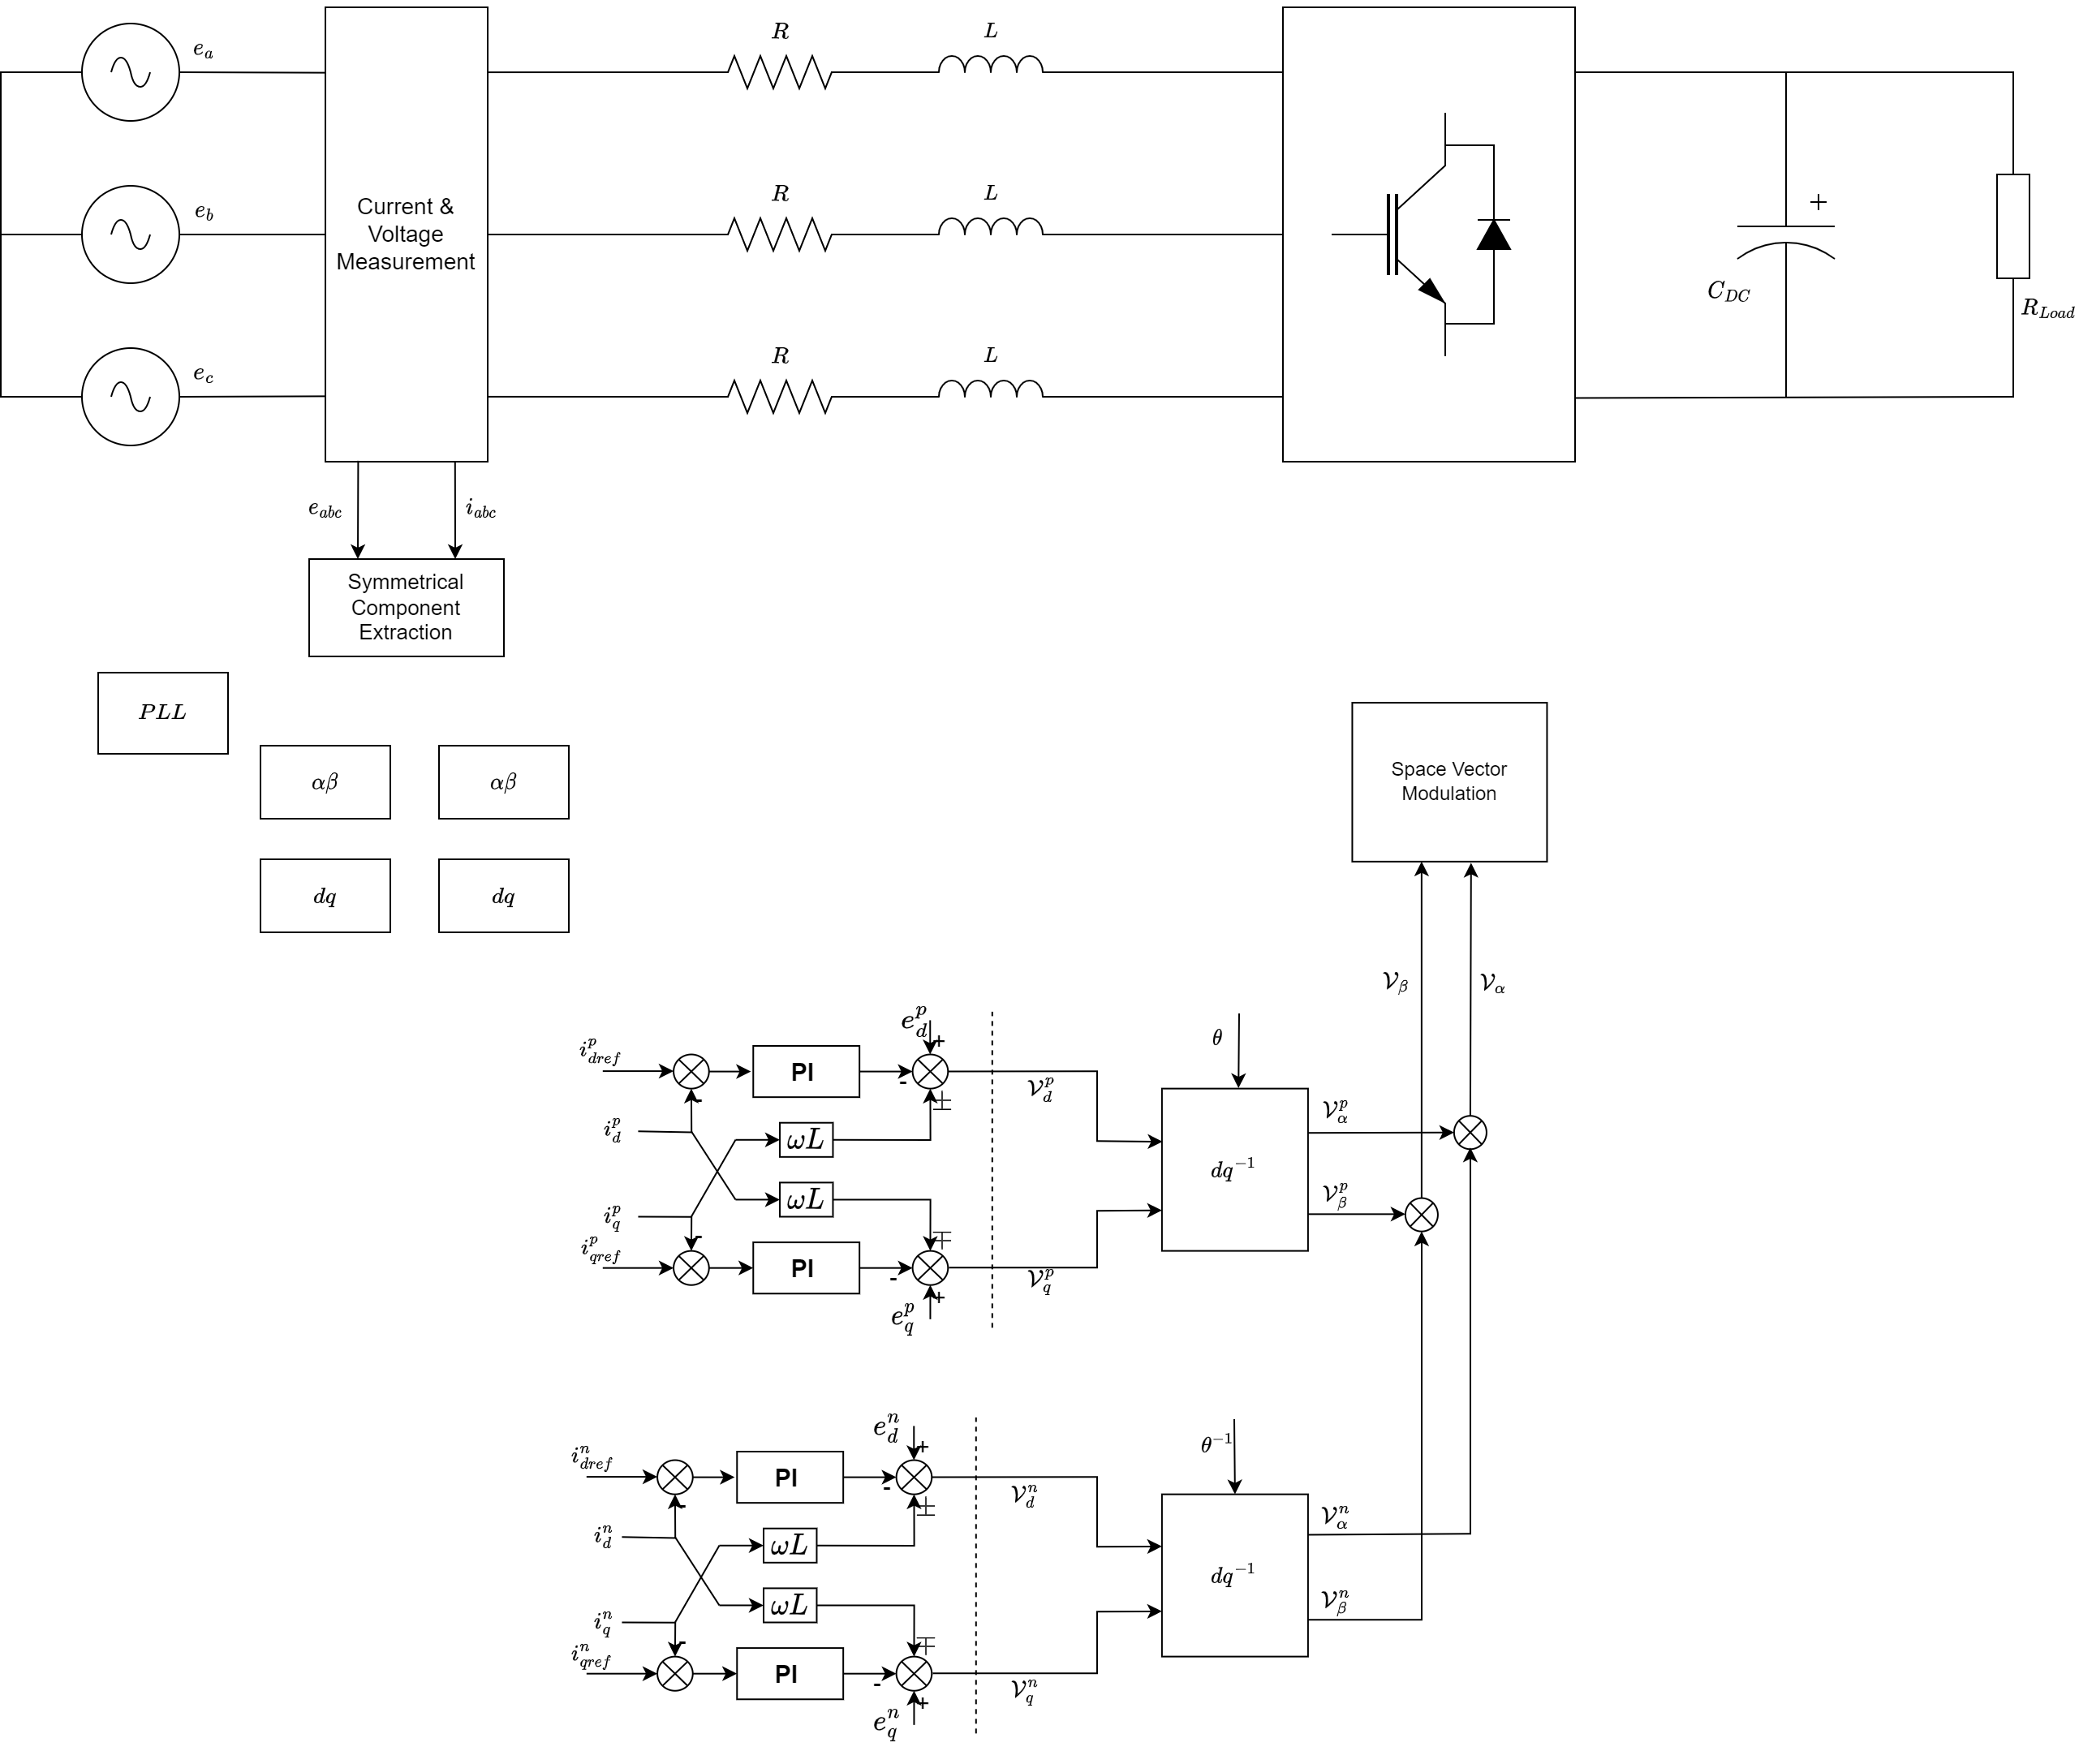
\includegraphics[width=\textwidth]{img/ControllerStructure.png}
        \end{figure}
    \end{columns}
\end{frame}

% 13. PI Current Controller Design
\begin{frame}{PI Current Controller Design}
    \begin{columns}
        \column{0.5\textwidth}
        The inner current control loop is designed using a standard PI structure with feedforward
        compensation to cancel the cross-coupling terms in the $d$-$q$ frame.
        \begin{equation*}
            \begin{split}
                \mathcal{V}_{d}^{p}    &= -\mathcal{U}_{d}^{p} + e_{d}^{p} + \omega L i_{q}^{p} \\
                \mathcal{V}_{q}^{p}    &= -\mathcal{U}_{q}^{p} + e_{q}^{p} - \omega L i_{d}^{p} \\
                \mathcal{V}_{d}^{n}    &= -\mathcal{U}_{d}^{n} + e_{d}^{n} - \omega L i_{q}^{n} \\
                \mathcal{V}_{q}^{n}    &= -\mathcal{U}_{q}^{n} + e_{q}^{n} + \omega L i_{d}^{n}        
            \end{split}
        \end{equation*}  

        \column{0.5\textwidth}
        \begin{figure}
            \centering
            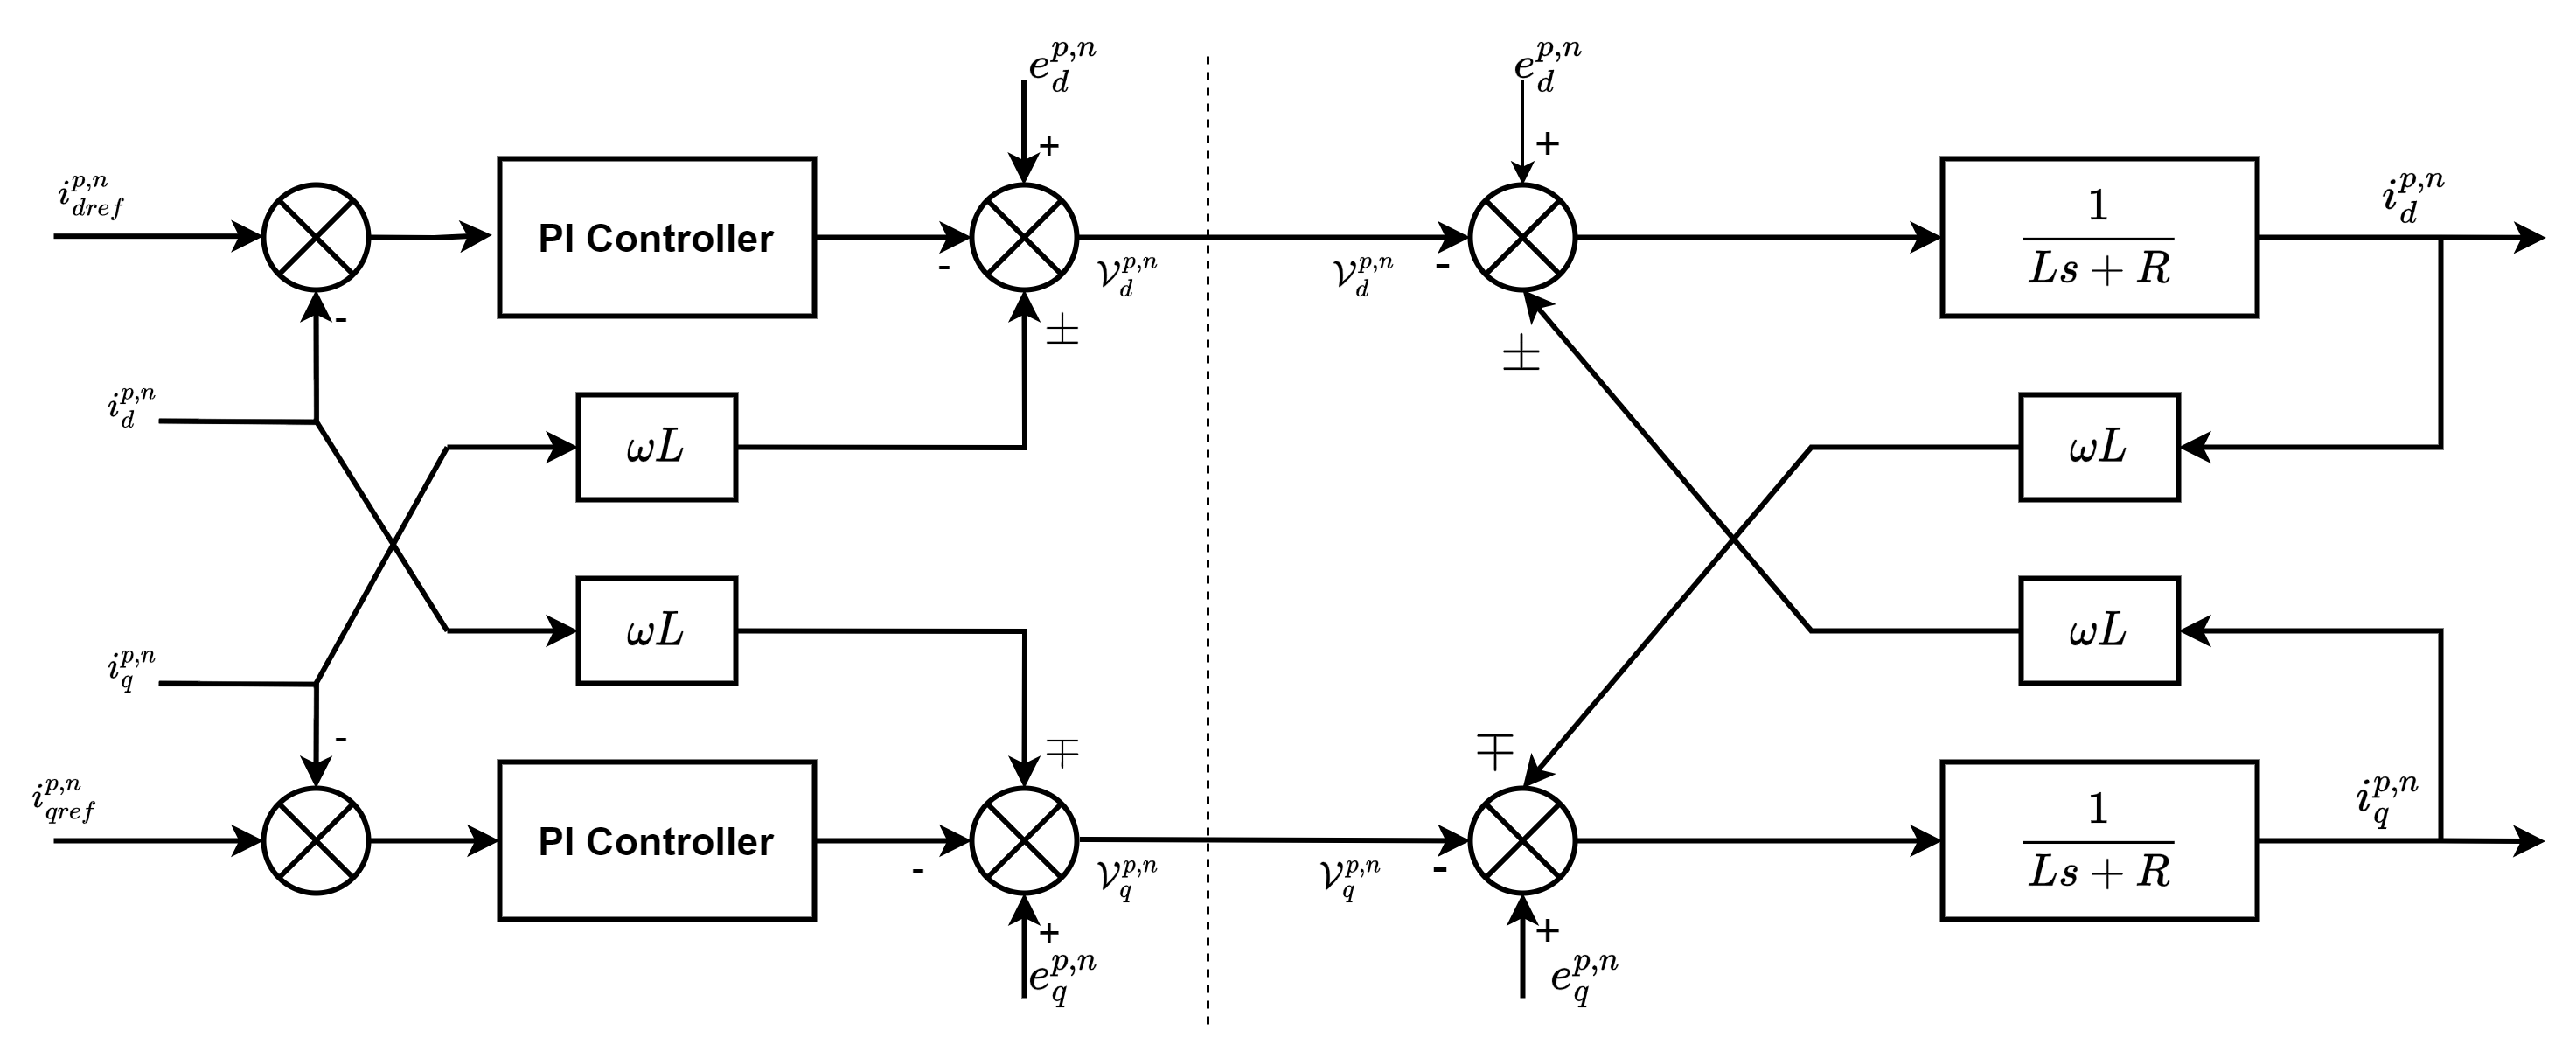
\includegraphics[width=\textwidth]{img/decoupledController.png}
        \end{figure}
    \end{columns}
\end{frame}

%14. PI Current Controller Design

\begin{frame}{PI Current Controller Design \dots(Cont'd)}
    The PI controller parameters are tuned using the Internal Model Control (IMC) method based on 
    the linearized system dynamics. 
    \begin{equation*}
        \begin{split}
            K_{p} &= \frac{L}{\tau_c} \\
            K_{i} &= \frac{R}{\tau_c}
        \end{split}
    \end{equation*}
    where $\tau_c$ is the desired closed-loop time constant, chosen to be at least ten times smaller than the
    switching frequency of the inverter to ensure that the controller can respond quickly enough to
    changes in the reference current.
    \begin{equation*}
        \tau_c = \frac{10}{2 \pi f_{s}}
    \end{equation*}
\end{frame}

% 15. MPC Cost Function Formulation
\begin{frame}{MPC: Cost Function Formulation}
    By defining the state variable $W = {V_{dc}}^{2}$ (Energy), the dynamics are linearized. 
    \begin{equation*}
        W(k+1) = W(k) + \frac{2 T_s}{C} \left( P_{in}(k) - P_{load}(k) \right)
    \end{equation*}

    The control input vector is defined as the current references:
    \begin{equation*}
        \mathbf{u}(k) = \begin{bmatrix} i_d^p(k) & i_q^p(k) & i_d^n(k) & i_q^n(k) \end{bmatrix}^T
    \end{equation*}

    The instantaneous power components are linearly related to the currents via the grid voltage matrix $\mathbf{G}(k)$:
    \begin{equation*}
        \mathbf{y}(k) = \begin{bmatrix} P_0(k) & Q_0(k) & P_{c2}(k) & P_{s2}(k) \end{bmatrix}^T = \mathbf{G}(k) \mathbf{u}(k)
    \end{equation*}
\end{frame}

% 16. MPC Cost Function Formulation
\begin{frame}{MPC: Cost Function Formulation \dots(Cont'd)}
    The future states of the DC energy over the full prediction horizon ($N_p$) are related to input vector by the modified prediction model:
    \begin{equation*}
        \mathbf{W}_{pred} = \mathbf{S}_x W(k) + \mathbf{S}_u \mathbf{U} + \mathbf{S}_d P_{load}(k)
    \end{equation*}
    where:
    \begin{itemize}
    \item $\mathbf{S}_x$: The free response vector (size $N_p \times 1$).
    \item $\mathbf{S}_u$: The forced response matrix (size $N \times 4N$).
    \item $\mathbf{S}_d$: The disturbance response vector (size $N_p \times 1$).
    \end{itemize}
    \vspace{0.3cm}
    The decision vector of unknown control inputs, $\mathbf{U}$, is:
    \begin{equation*}
        \mathbf{U} = [\mathbf{u}(k)^T, \mathbf{u}(k+1)^T, \dots, \mathbf{u}(k+N_c-1)^T]^T
    \end{equation*}
\end{frame}
% ---------------------------------------------------------
\section{Simulation Results}
% ---------------------------------------------------------

% 10. Type B Fault Response
\begin{frame}{Simulation Results: Unbalanced Grid (Type B Fault)}
    \begin{columns}
        \column{0.4\textwidth}
        \begin{itemize}
            \item Introduction of a Type B voltage sag (magnitude reduction).
            \item The MPC algorithm successfully suppresses the $2\omega$ ripple on the DC link.
            \item Current references deliberately distort to compensate for the negative sequence voltage.
        \end{itemize}
        
        \column{0.6\textwidth}
        \begin{figure}
            \centering
            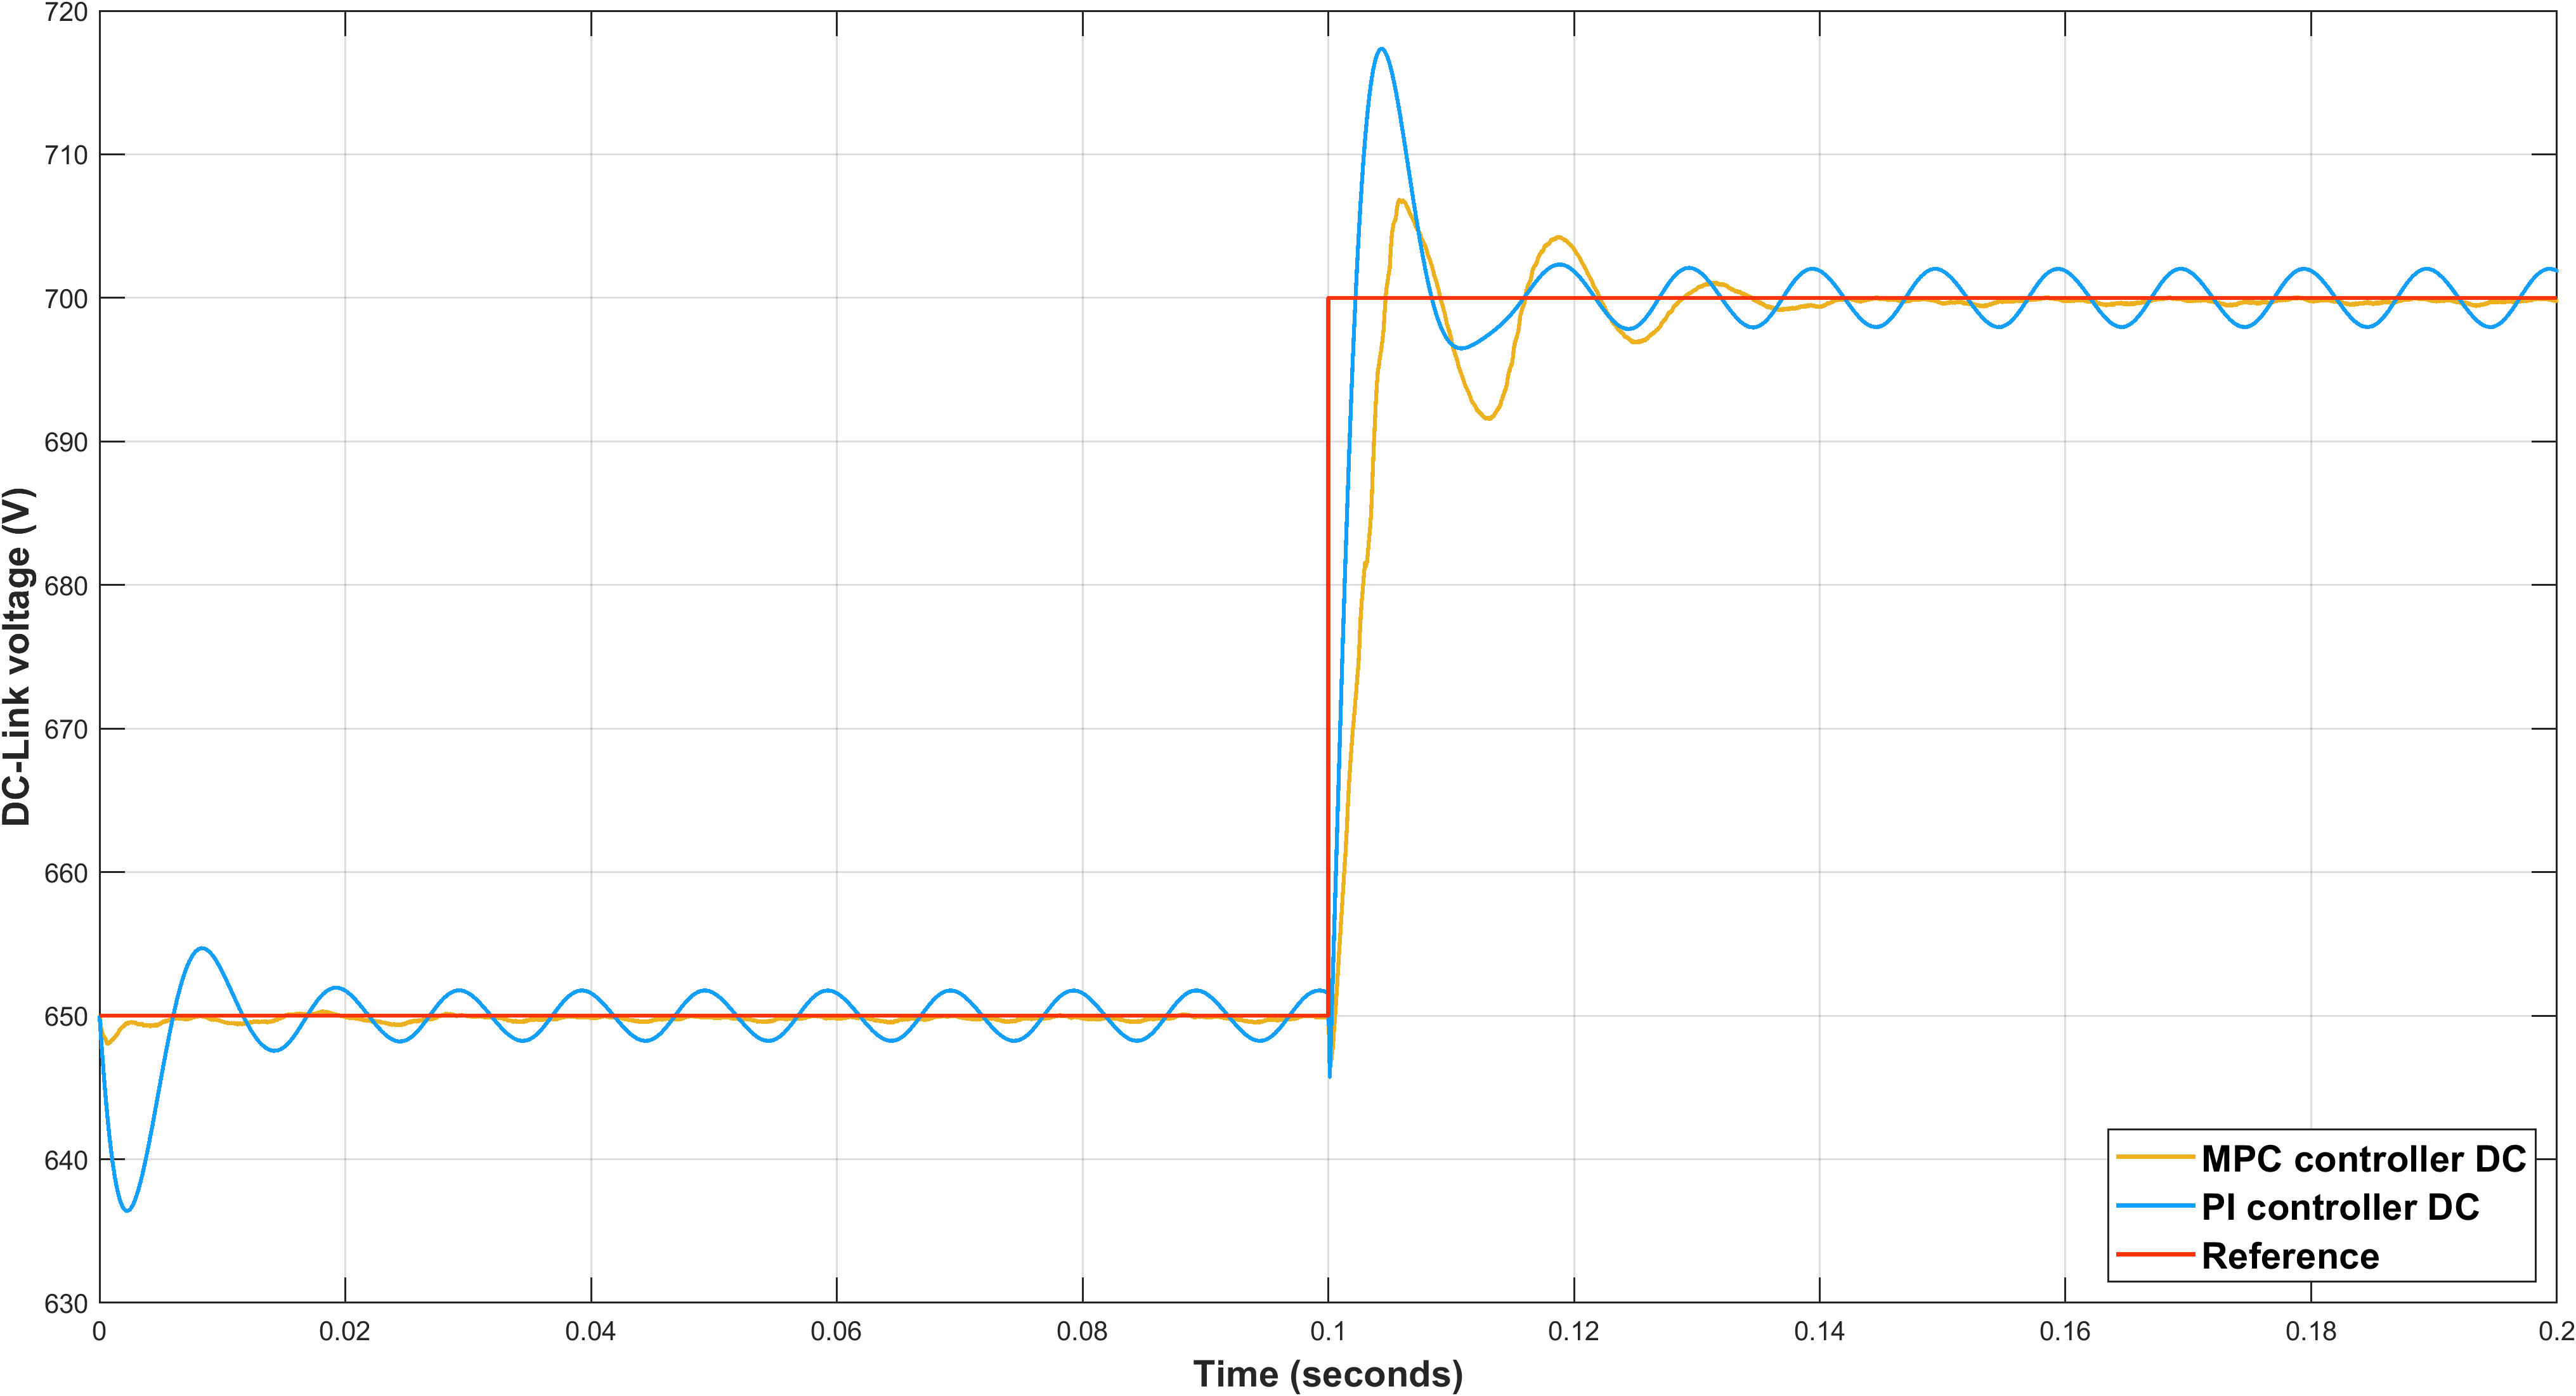
\includegraphics[width=0.8\textwidth]{img/TypeB_voltage_Vdc.png}\\
            \vspace{0.2cm}
            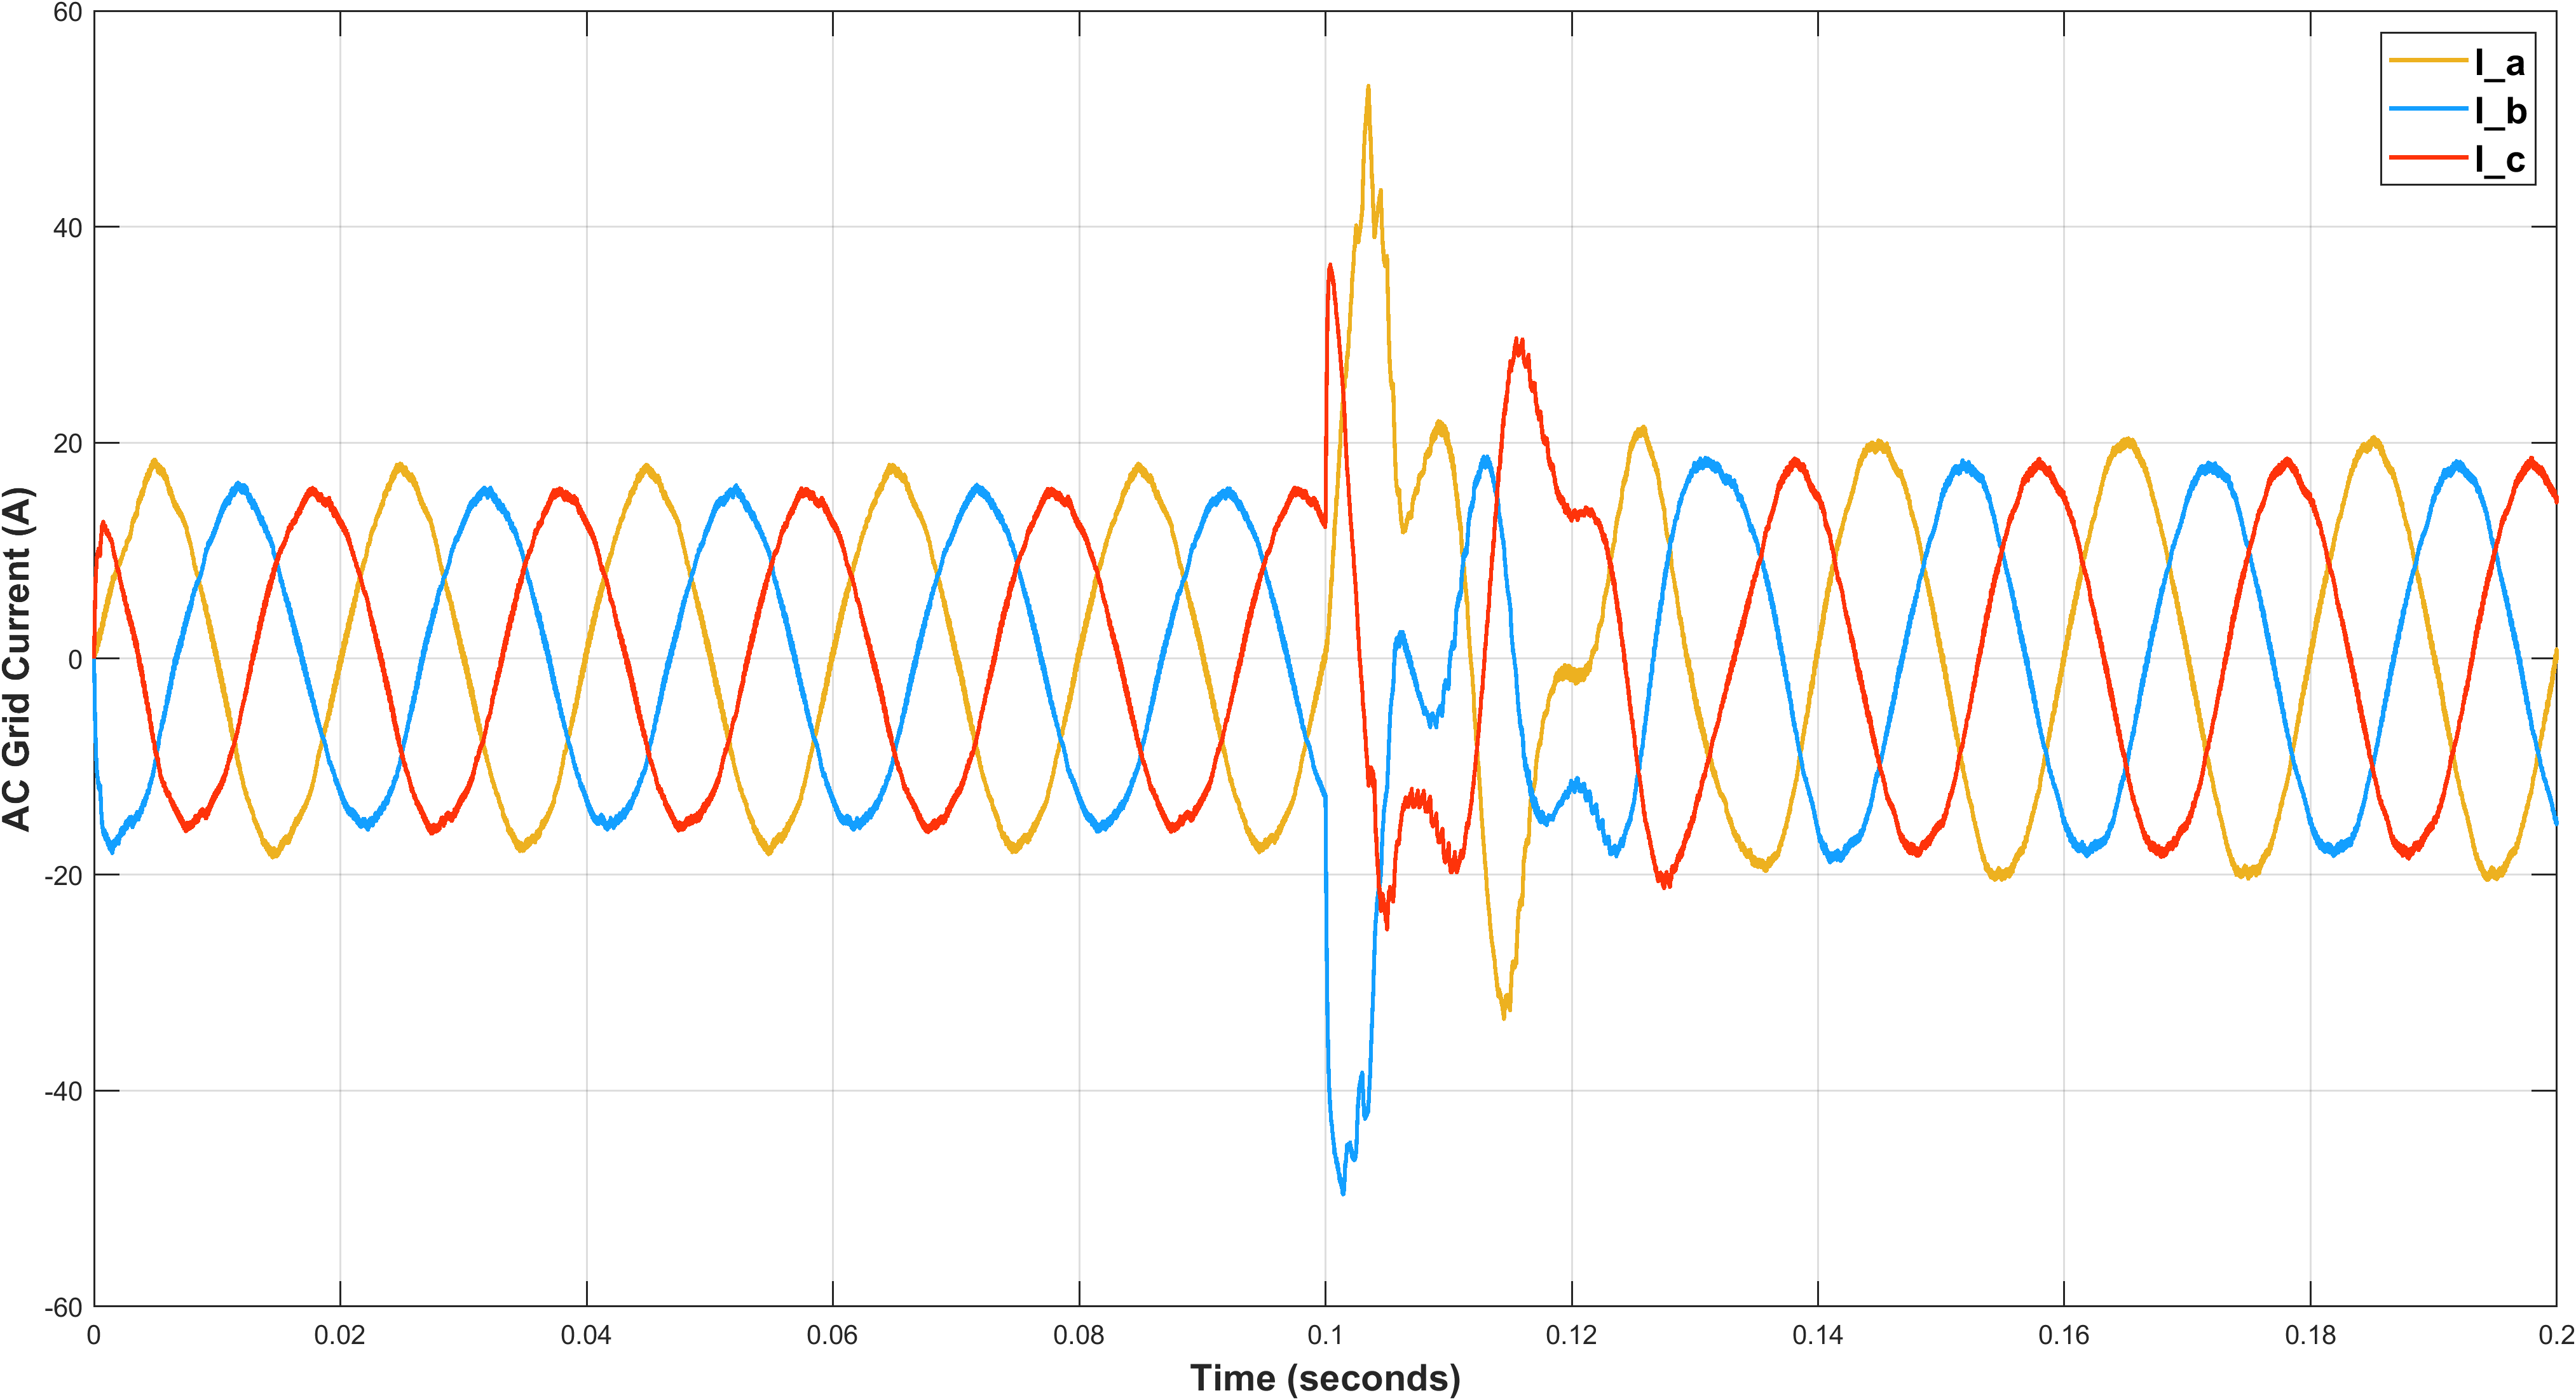
\includegraphics[width=0.8\textwidth]{img/TypeB_current_abc.png}
        \end{figure}
    \end{columns}
\end{frame}

% 11. Type F Fault Response
\begin{frame}{Simulation Results: Severe Unbalance (Type F/G Fault)}
    \begin{columns}
        \column{0.4\textwidth}
        \begin{itemize}
            \item Under severe multi-phase unbalance (significant phase shifts and sags).
            \item DC Voltage remains stable.
            \item THD remains $< 3.5\%$ for all phases, ensuring unity power factor.
        \end{itemize}
        
        \column{0.6\textwidth}
        \begin{figure}
            \centering
            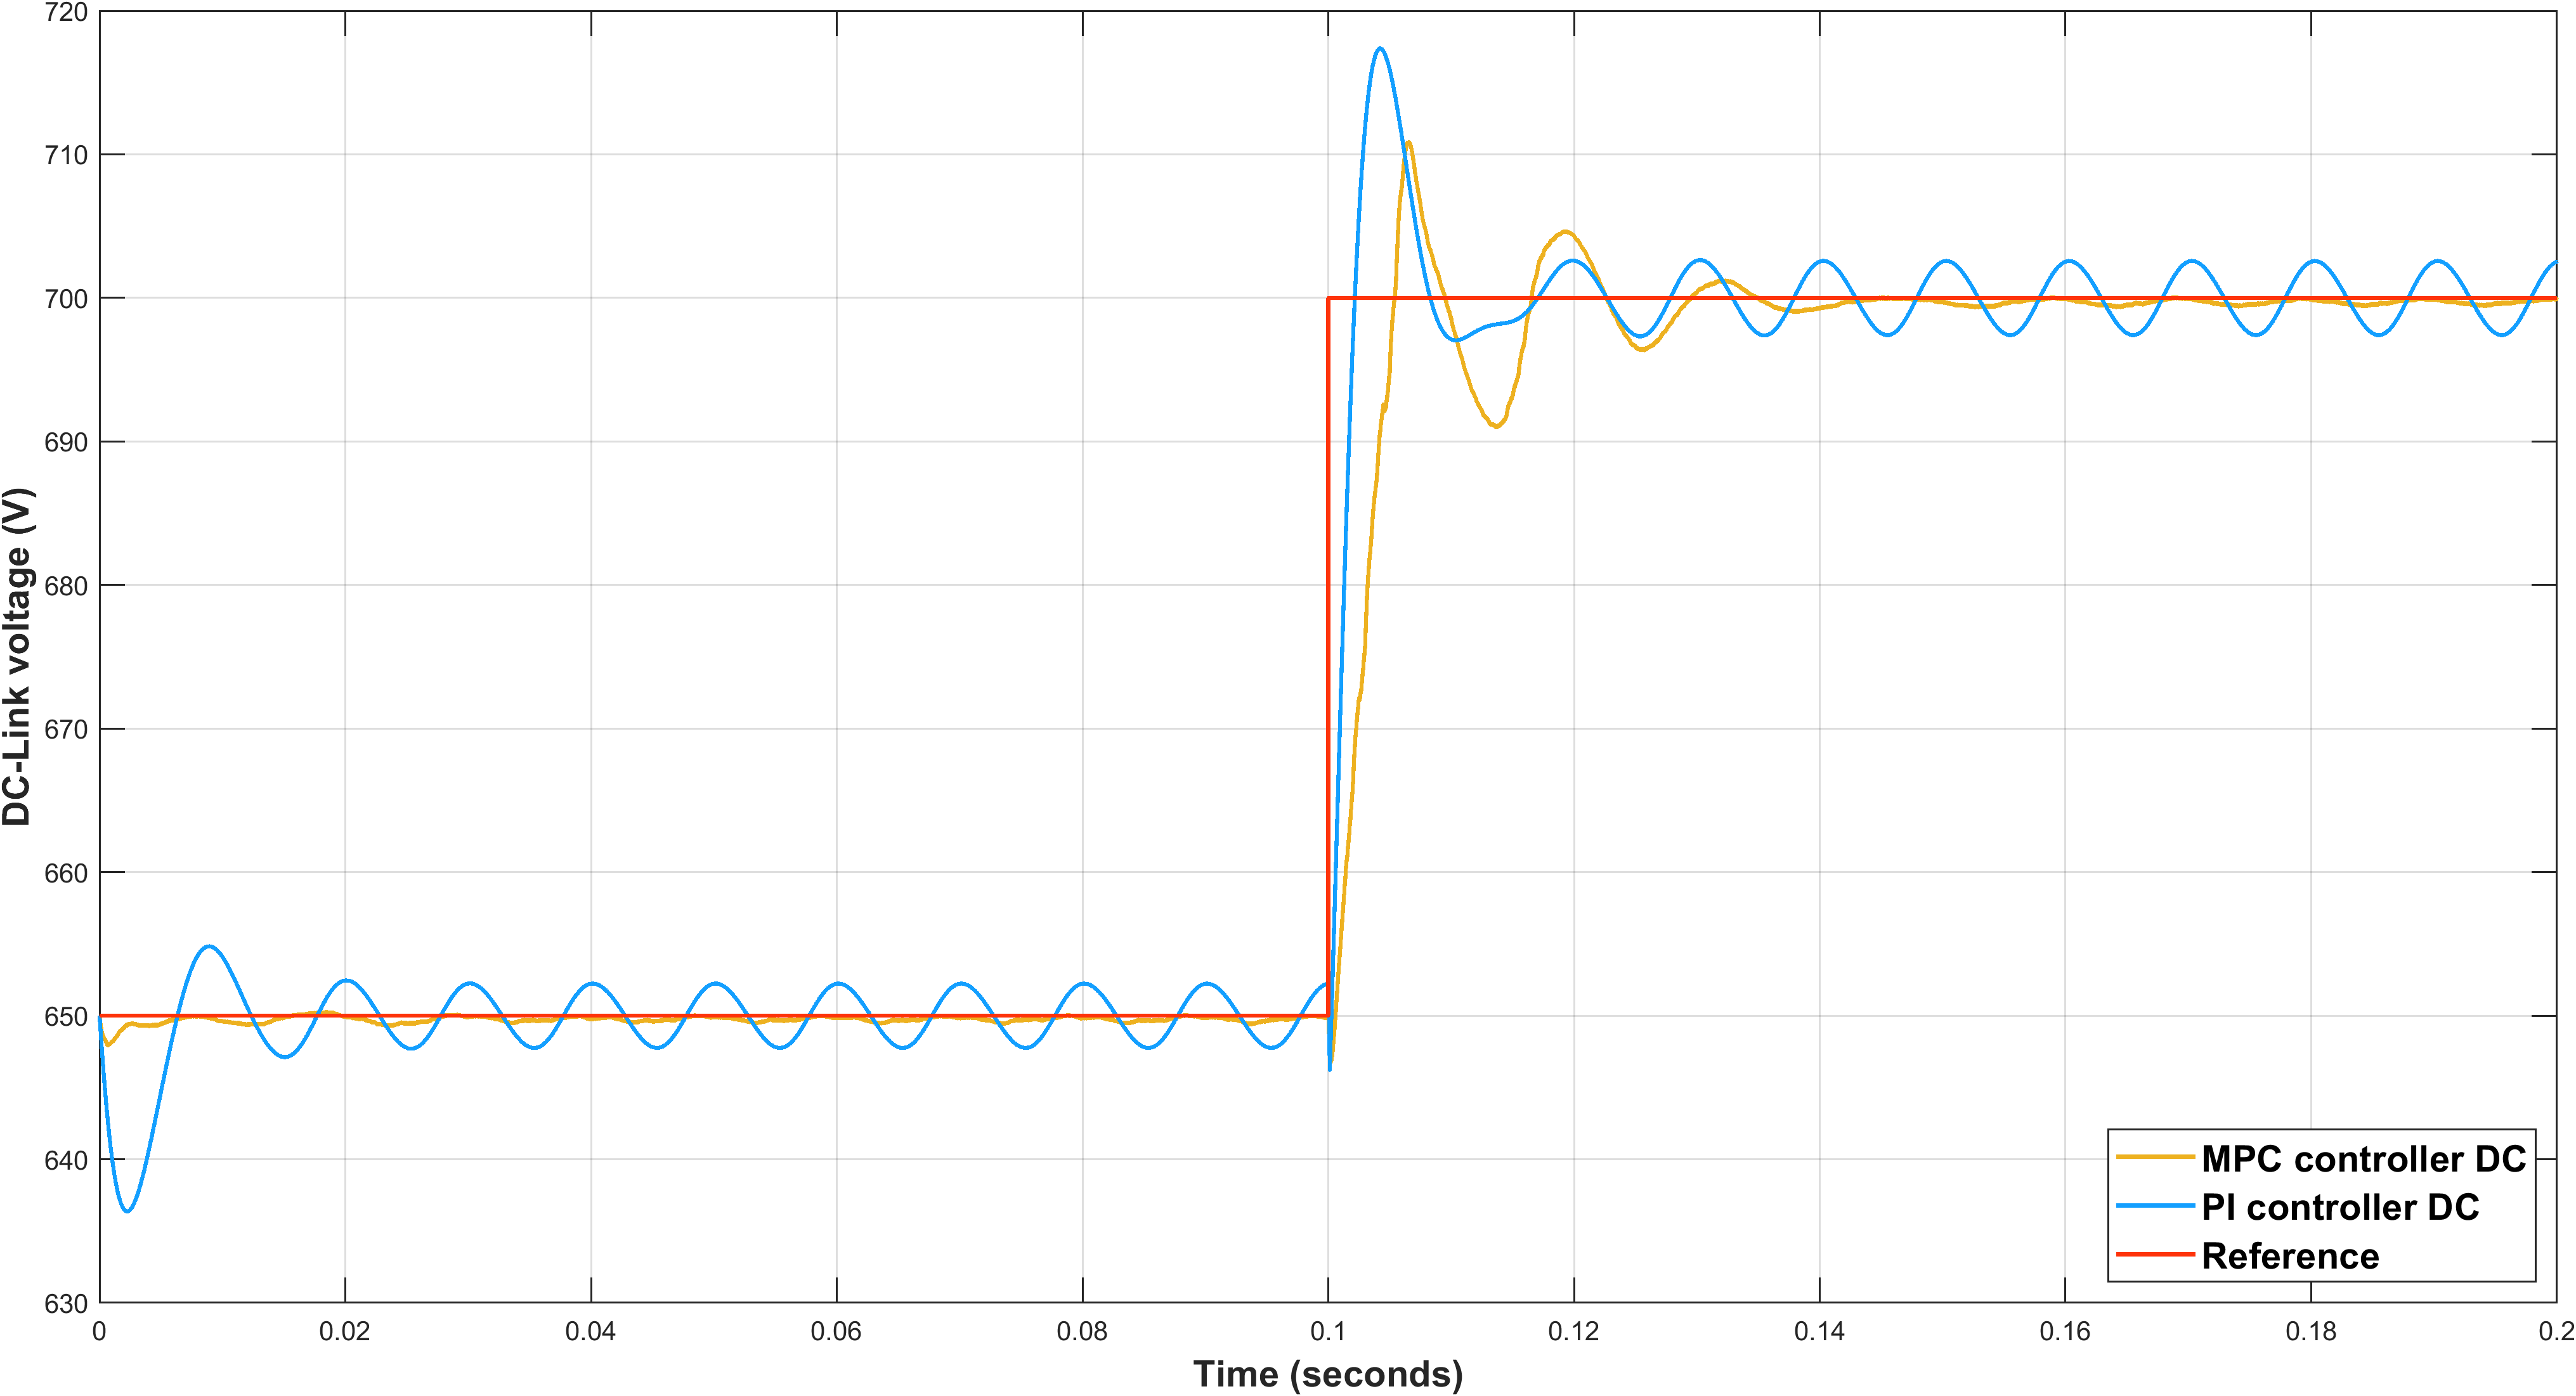
\includegraphics[width=0.8\textwidth]{img/TypeF_voltage_Vdc.png}\\
            \vspace{0.2cm}
            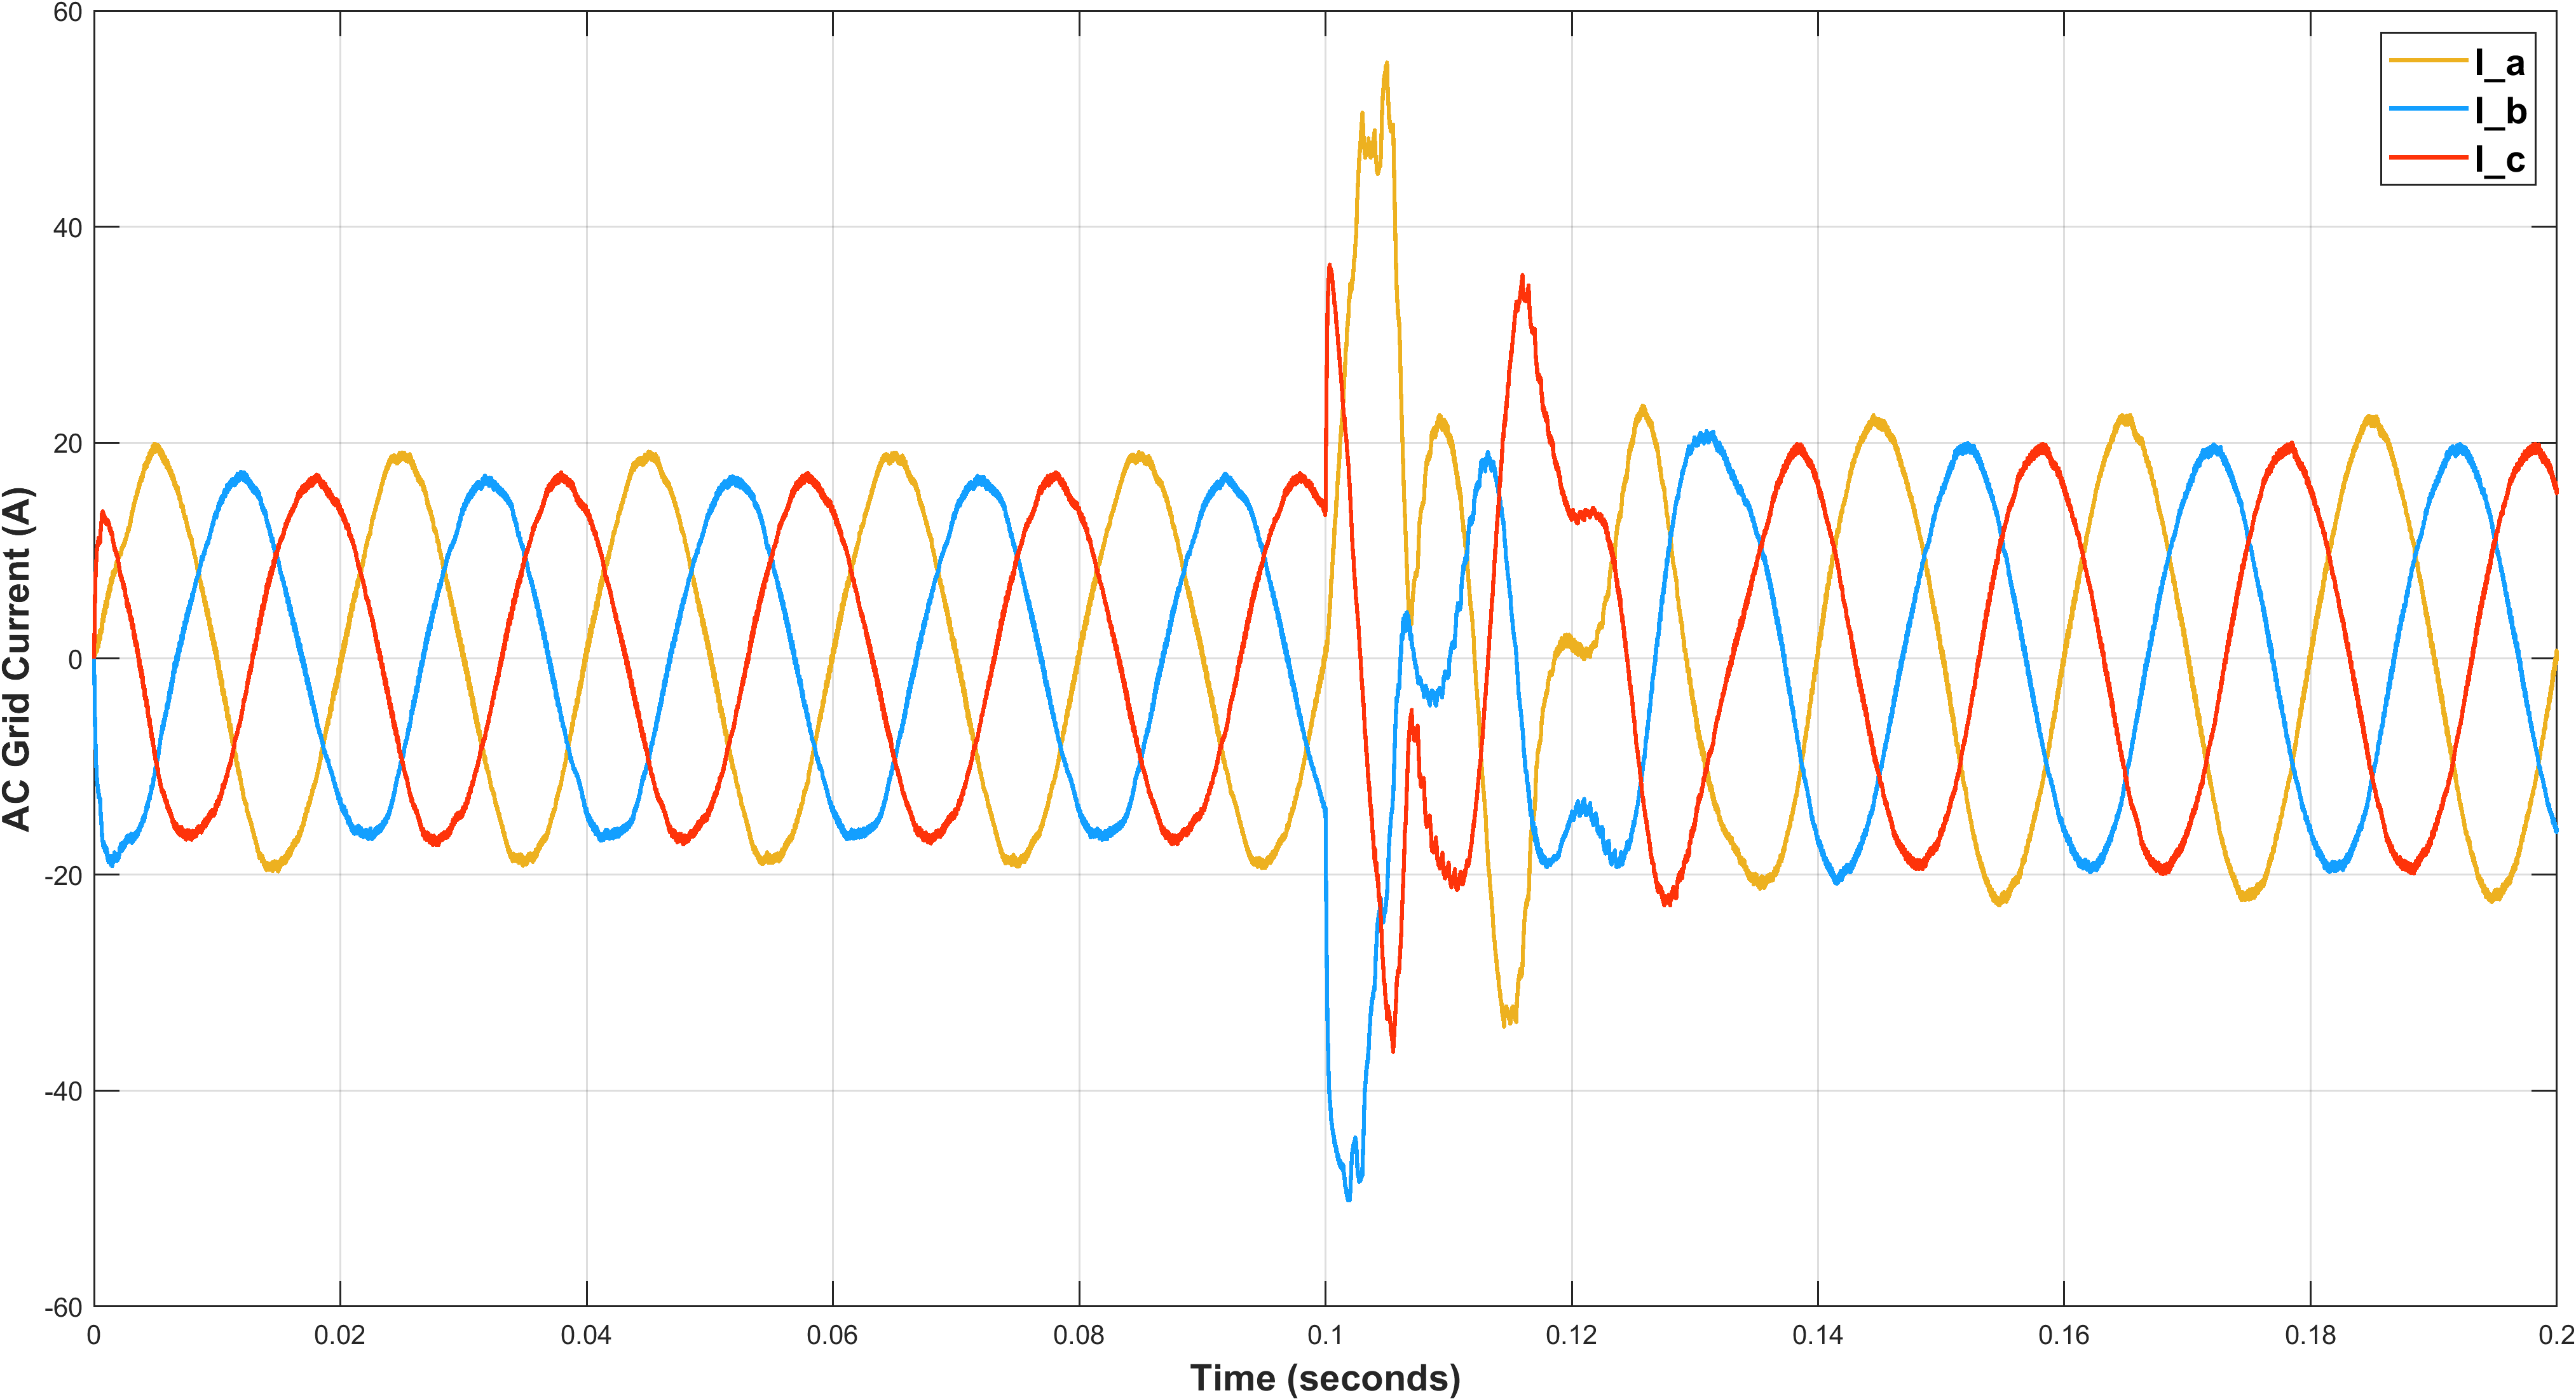
\includegraphics[width=0.8\textwidth]{img/TypeF_current_abc.png}
        \end{figure}
    \end{columns}
\end{frame}

% ---------------------------------------------------------
\section{Conclusion}
% ---------------------------------------------------------

% 12. Conclusion
\begin{frame}{Conclusion}
    \begin{itemize}
        \item The MPC Strategy effectively mitigates DC ripples caused by negative sequence voltage components.
        \item Linearization using the Energy state (${V_{dc}}^{2}$) significantly improves tracking stiffness.
        \item The cascaded loop structure achieves fast dynamic response while maintaining low switching losses and high power quality.
    \end{itemize}
\end{frame}

% 13. Q&A Slide
\begin{frame}
    \begin{center}
        {\Huge \textbf{Thank You!}} \\
        \vspace{1cm}
        {\Large \textbf{Questions?}} \\
        \vspace{1cm}
        {\normalsize kibrom.esayas@mu.edu.et | Mekelle University}
    \end{center}
\end{frame}

\end{document}